%%% fs-seim-experiments - Experiments

\label {fs-experiments}

\subsection{Setup}
We performed the series of experiments to estimate the performance of our system's prototype. As a stream processing task, we apply building an inverted index. This task is chosen because it has the following properties:

\begin{enumerate}
    \item Task requires stateful operations. It allows us to check the performance of the proposed stateful pipeline
    \item Computational flow of the task contains network shuffle that can violate the ordering constraints of some operations. Therefore, inverted index task can verify the performance of our optimistic approach
    \item The load distribution is skewed, because of Zipf's law
\end{enumerate}

These properties make the task sufficient to comprehensively analyze the performance of the proposed solution. Building inverted index can be considered as the halfway task between documents generation and searching. In the real-world, such scenario can be found in freshness-aware systems, e.g., news processing engines.

The logical pipeline of this computation is shown in Figure ~\ref{inverted-index}. First map operation accepts Wikipedia documents and outputs pairs of words and corresponding positions. The next part of the pipeline accepts pairs of word and positions and computes updated posting list and the actual changelog. 

This stateful transformation is implemented in the form of groping and map operation with a cycle, as it was shown in the previous section. Regarding the physical deployment, the full logical graph is deployed on each computational unit or worker. Documents are randomly shuffled before the first map operation. Word positions are partitioned by word before grouping. The other links are implemented as simple chain calls.

\begin{figure}[htbp]
  \centering
  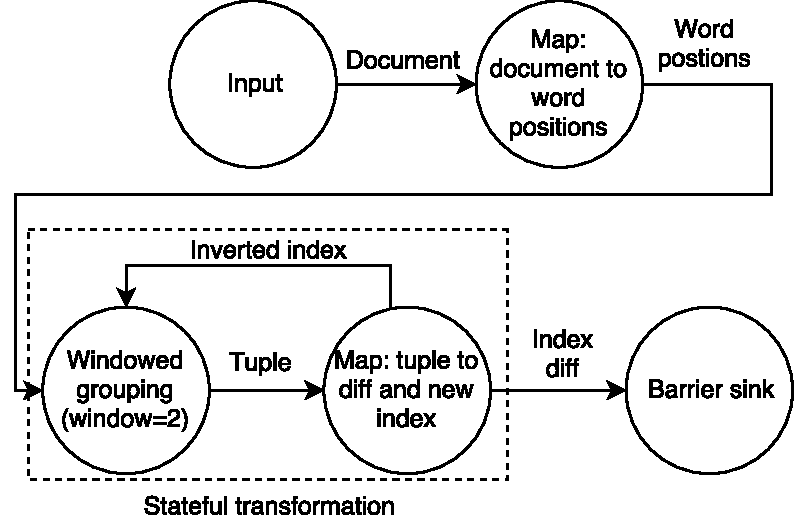
\includegraphics[width=0.48\textwidth]{pics/inverted-index}
  \caption{Logical pipeline for inverted index}
  \label {inverted-index}
\end{figure}

Our experiments were performed on clusters of 10 nodes. Each node is an AWS EC2 micro instance with 1GB RAM and 1 core CPU.

\subsection{Overhead and scalability}

As a key metric in our experiment, we take the ratio of arrived at the barrier items count to the number of the valid items among them. This value clearly represents the overhead of our approach, as it was mentioned at the end of the previous section. 

The relation between the number of workers, the delay between input documents and the proposed ratio is shown in Figure ~\ref{experiment}. As expected, the peak of the ratio is achieved when the document per second rate is high, and the number of the nodes is low. This behavior can be explained by the fact that a few workers cannot effectively deal with such intensive load. Nevertheless, the proportion of invalid items reduces with the increase of workers number. Under non-extreme load, the total overhead of the optimistic approach is under 10\% for all considered number of workers. These results confirm that the ratio does not increase with the growth of the number of nodes.

Therefore, the most important conclusions of the experiments are: the proposed method is scalable, the overhead could be optimized by system setup.

%% TODO: 
\begin{figure}[htbp]
  \centering
  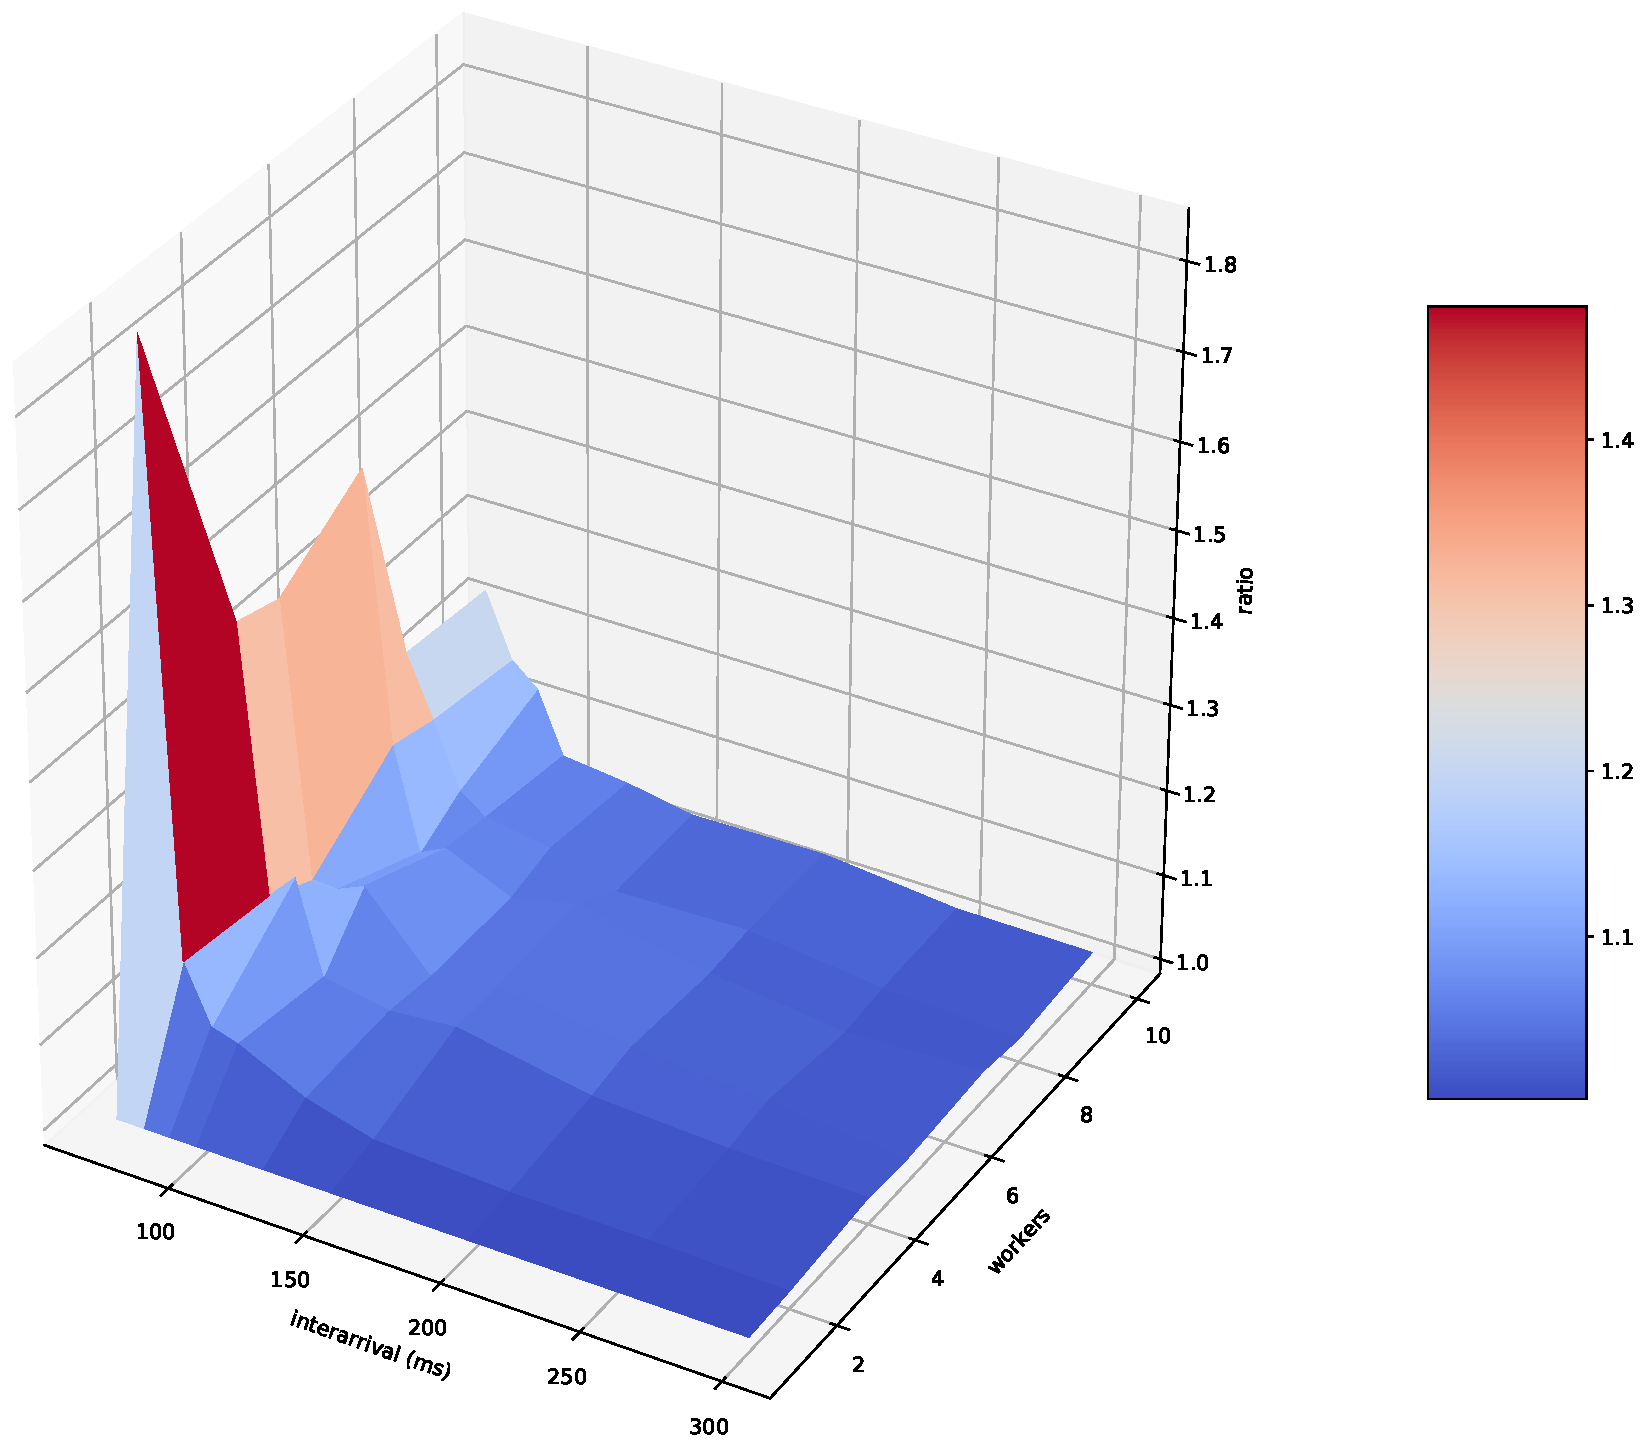
\includegraphics[width=0.5\textwidth]{pics/experiment}
  \caption{The relation between the number of workers, the delay between input documents and the replay ratio}
  \label {experiment}
\end{figure}

\subsection{Comparison against Apache Flink}

We compared the performance of our optimistic approach with state-of-the-art stream processing system Apache Flink~\cite{carbone2015apache}. For Apache Flink, the algorithm for building the inverted index is adopted by the usage of {\it FlatMapFunction} for map step and stateful {\it RichMapFunction} for reduce step and for producing the change records. Order enforcing before reduce is implemented using custom {\it ProcessFunction} that buffers all input until corresponding low watermark is received. Watermarks are sent after each document. The network buffer timeout is set to 0 to minimize latency. 

In this paper, we compare $50^{th}$, $75^{th}$, $95^{th}$, and $99^{th}$ percentile of distributions, which clearly represent the performance from the perspective of the users' experience.

The comparison of latencies between \FlameStream\ and Flink within 10 nodes and distinct document rates is shown in Figure~\ref{fs-index-quantiles}. In this case, \FlameStream\ provides lower latency even under high load. These results confirm that optimistic approach for deterministic processing is able to provide less latency than conservative methods. Firstly, the reason for better performance can be the fact that Flink starts to update index only after the buffer before reduce stage is flushed. In contrast, \FlameStream\ flushes its barrier right before data is sent to a user, according to its optimistic nature. At this moment, all corresponding computations have been already done. Secondly, low watermarks go along the stream and can be delayed by long-running operations, while acker processes ack messages independently. It is confirmed by Figure~\ref{buffer-vs-barrier}, which shows the comparison between waiting time in Flink's buffer and \FlameStream's barrier.

\begin{figure}[htbp]
  \centering
  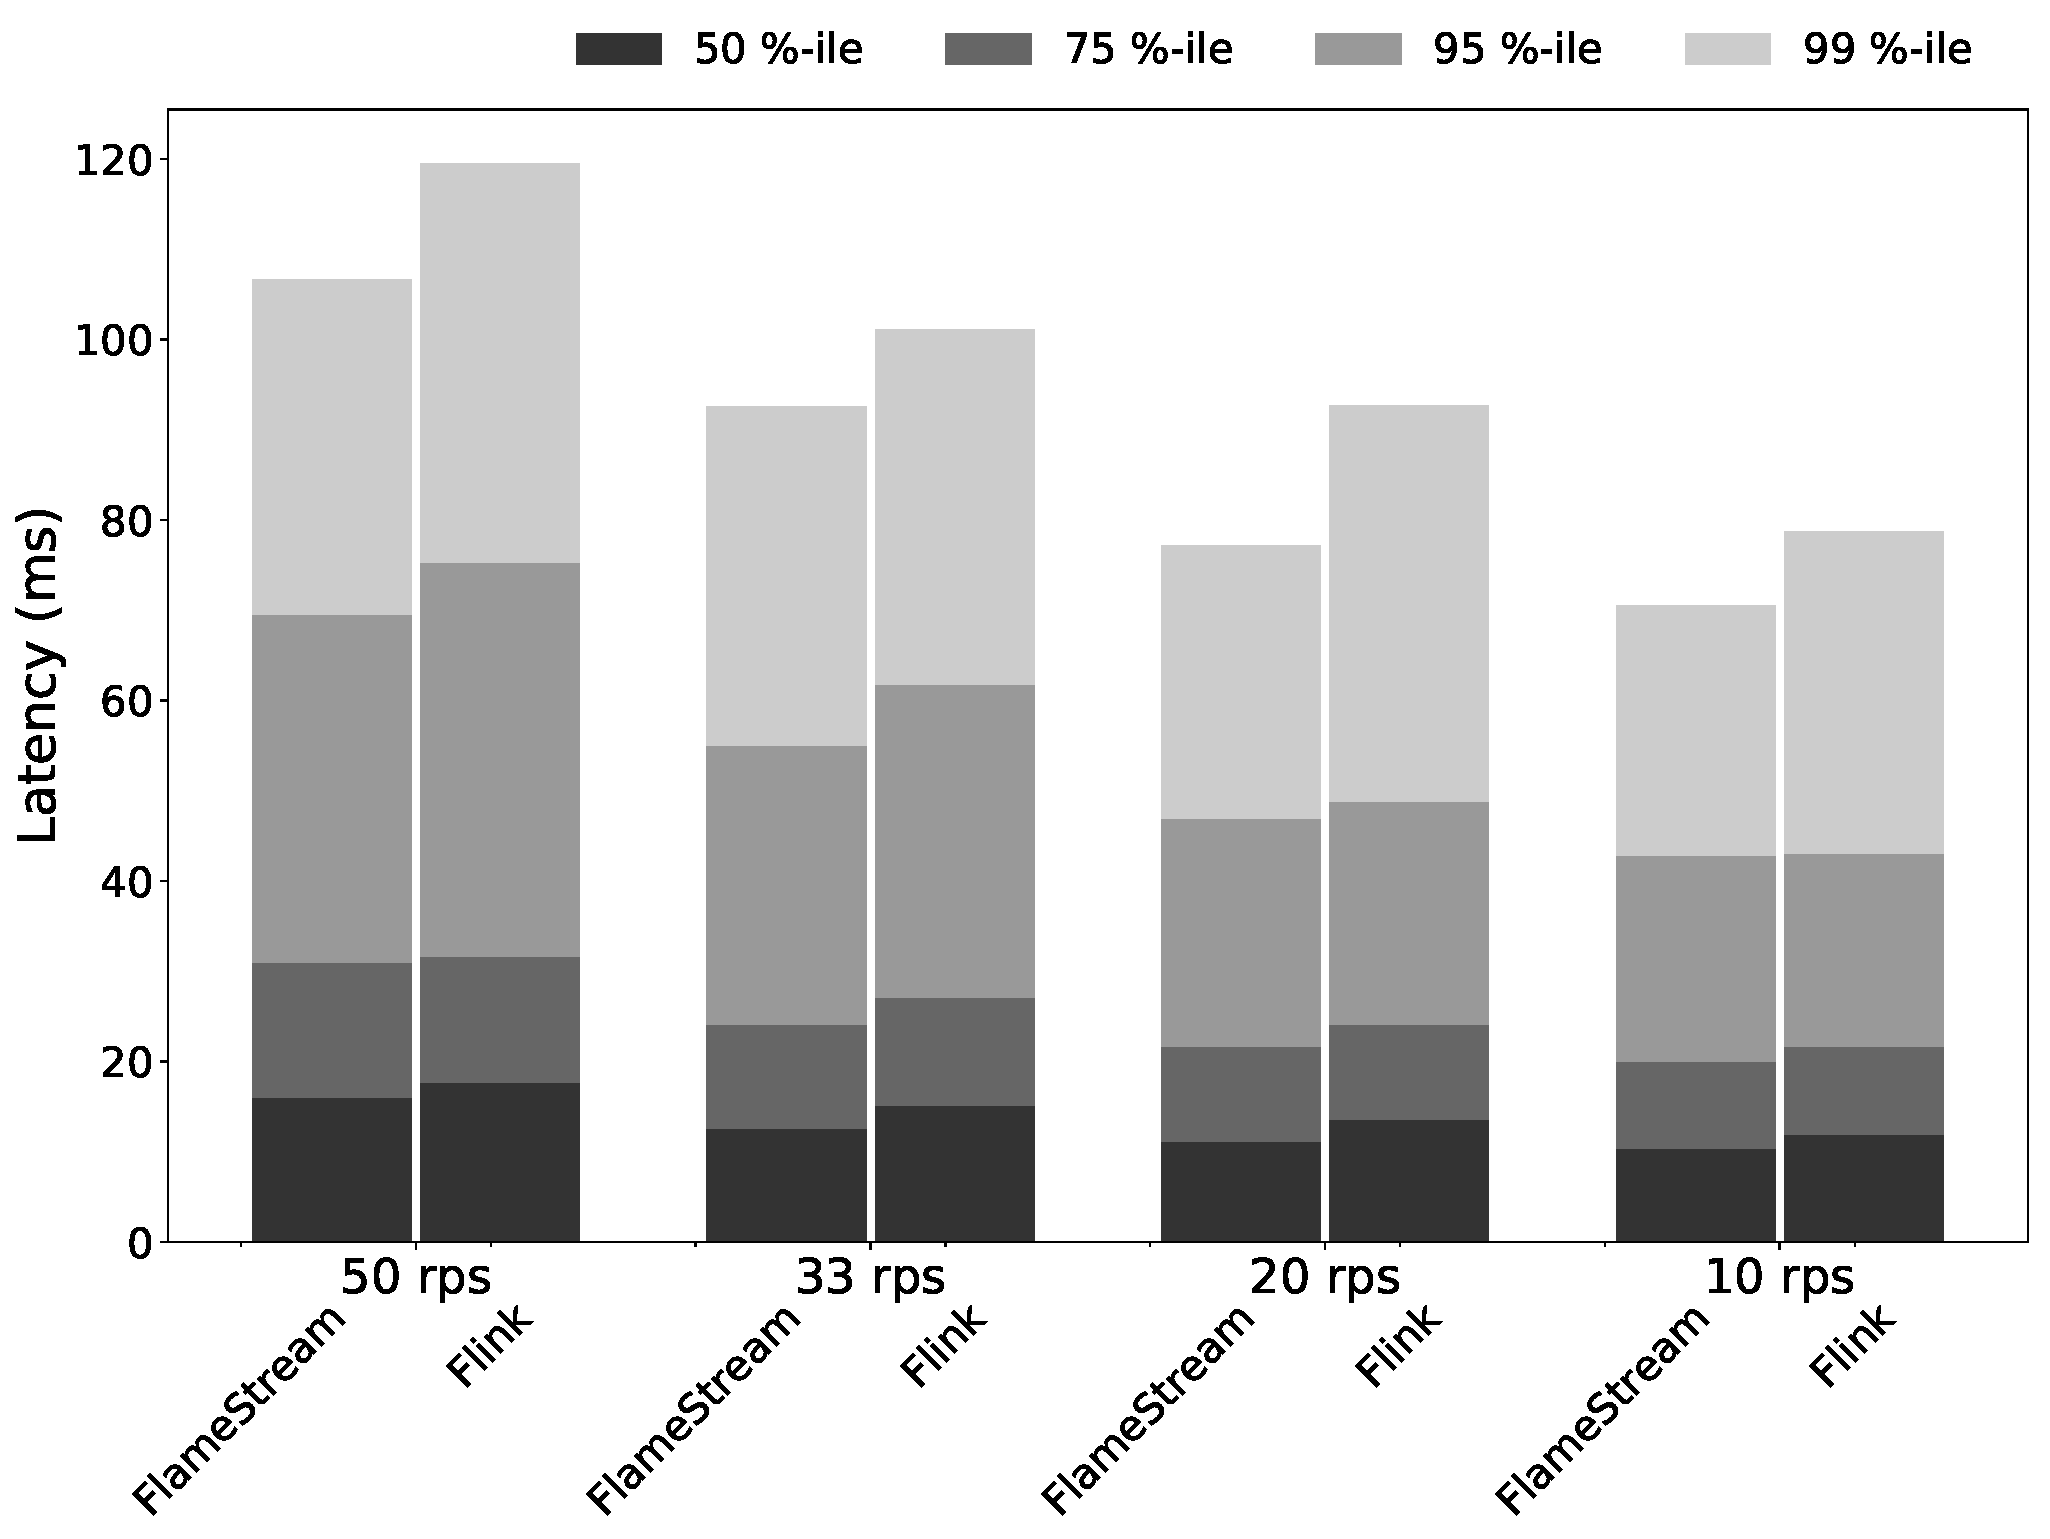
\includegraphics[width=0.47\textwidth]{pics/comp-index-quantiles}
  \caption{The comparison in latencies between \FlameStream\ and Flink within 10 nodes and distinct document rates}
  \label {fs-index-quantiles}
\end{figure}

\begin{figure}[htbp]
  \centering
  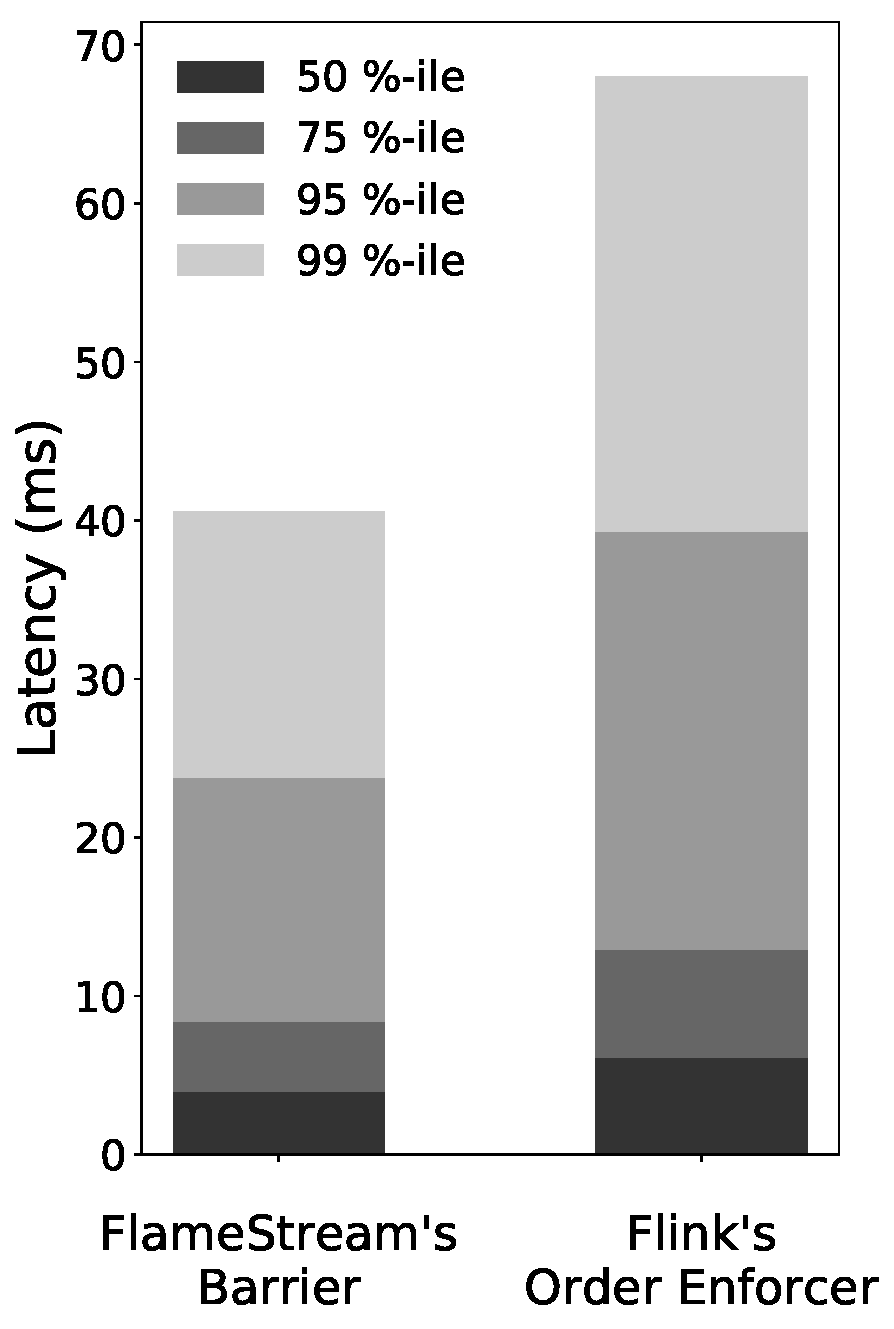
\includegraphics[width=0.20\textwidth]{pics/buffer-vs-barrier}
  \caption{Comparison between waiting time in Flink's buffer and FlameStream's barrier}
  \label {buffer-vs-barrier}
\end{figure}

However, there are conditions, which are not suitable for the optimistic approach. Figure~\ref{fs-index-quantiles-5} shows the comparison of latencies between \FlameStream\ and Flink within 5 nodes and distinct document rates. Flink outperforms \FlameStream\ under extreme load. Such behavior follows from the fact that \FlameStream\ provides significant overhead under very high pressure within a few computational units. This result evidently corresponds with measurements of the overhead in Figure~\ref{experiment}. Nevertheless, it should be noted that \FlameStream\ demonstrates better latency under non-extreme load.

\begin{figure}[htbp]
  \centering
  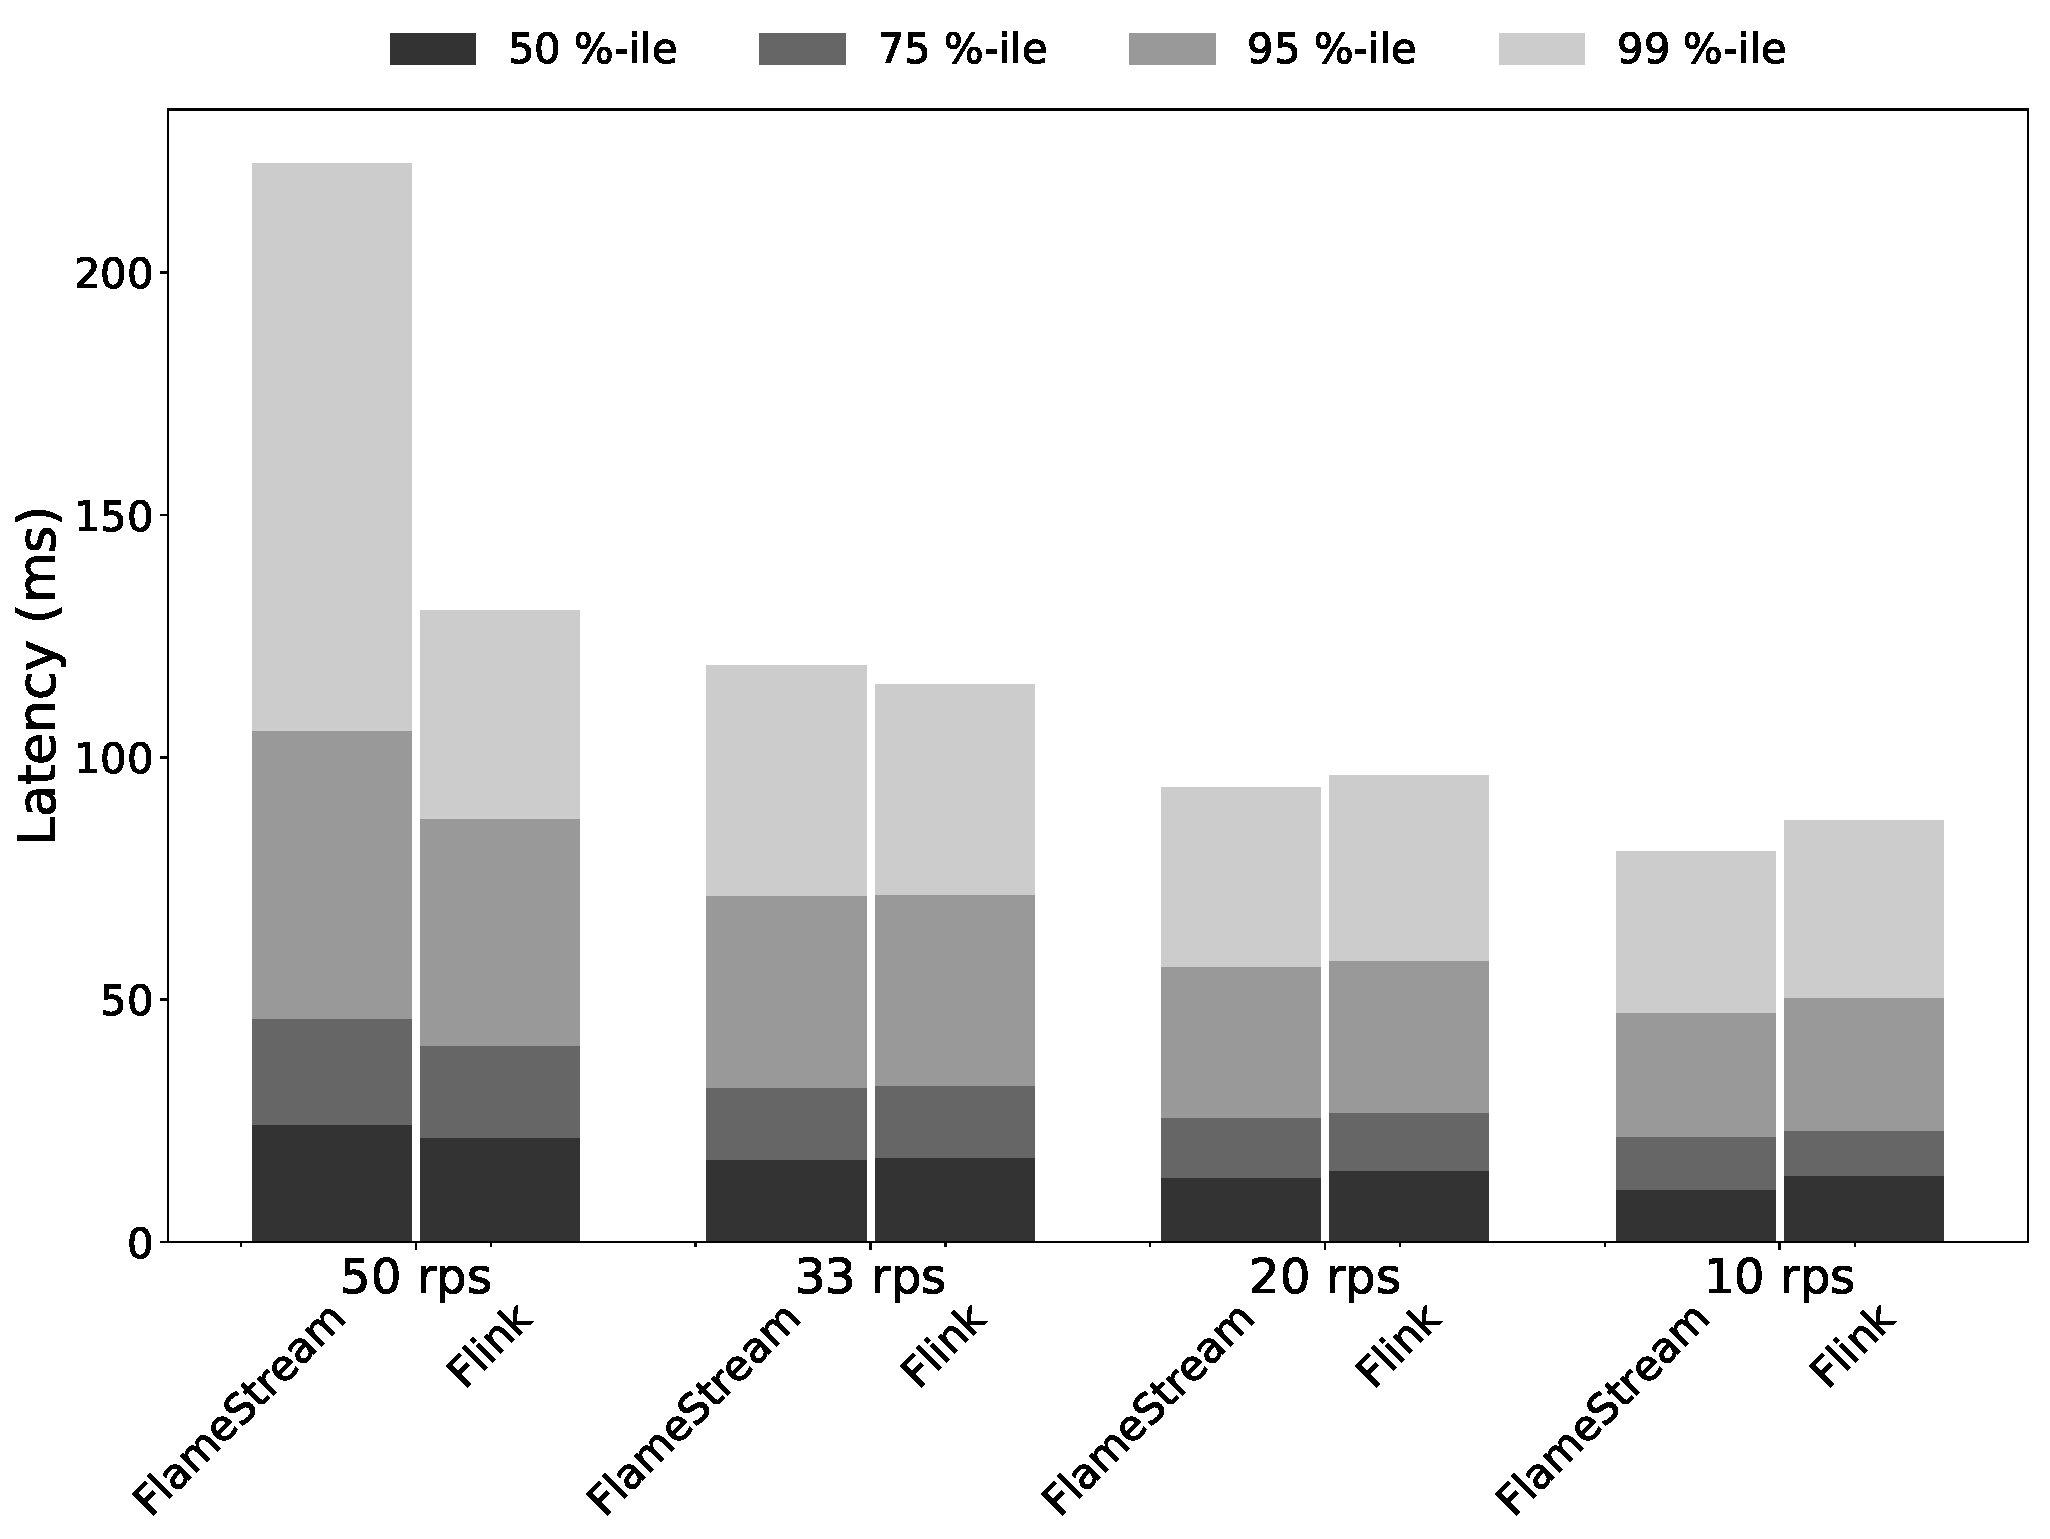
\includegraphics[width=0.47\textwidth]{pics/comp-index-quantiles_5}
  \caption{The comparison in latencies between \FlameStream\ and Flink within 5 nodes and distinct document rates}
  \label {fs-index-quantiles-5}
\end{figure}

Thus, Flink can be more appropriate if there is a need to optimize computational resources under a fixed load, but the demands on latency are not very strict, or determinism is not required. \FlameStream\ is more relevant for cases when low latency and determinism are strict requirements, but an allocation of additional resources is not a problem.  

